\chapter{Infraestructura}\label{cap.infraestructura}
En este capítulo se explicarán los principales ingredientes software en los que nos hemos apoyado para desarrollar el trabajo. Tales como el simulador Gazebo (con el cual se pueden simular robots con sus sensores y actuadores), el entorno JdeRobot, la biblioteca de OpenCV (empleada en todo lo relacionado con el tratamiento de imagen), PyQt (para el desarrollo de la interfaz gráfica) y Python como lenguaje de programación.

\section{Simulador Gazebo}

Como se argumentó en el Capítulo 1, el simulador Gazebo es uno de los ejes principales de JdeRobot-Academy. Es un simulador usado en robótica que permite realizar diversos escenarios tridimensionales donde probar nuestro software. A la hora de desarrollar el software es necesario hacer pruebas, las cuales saldrían muy costosas si se probaran en robots reales (podría no funcionar correctamente y que el robot se rompiera). Por esta razón es muy útil el empleo de simuladores, pues se pueden realizar las pruebas que se quieran sin peligro de que el robot se estropee. Con los simuladores se pueden diseñar robots y escenarios realistas donde ejecutar los algoritmos creados.

\begin{figure}[H]
  \begin{center}
    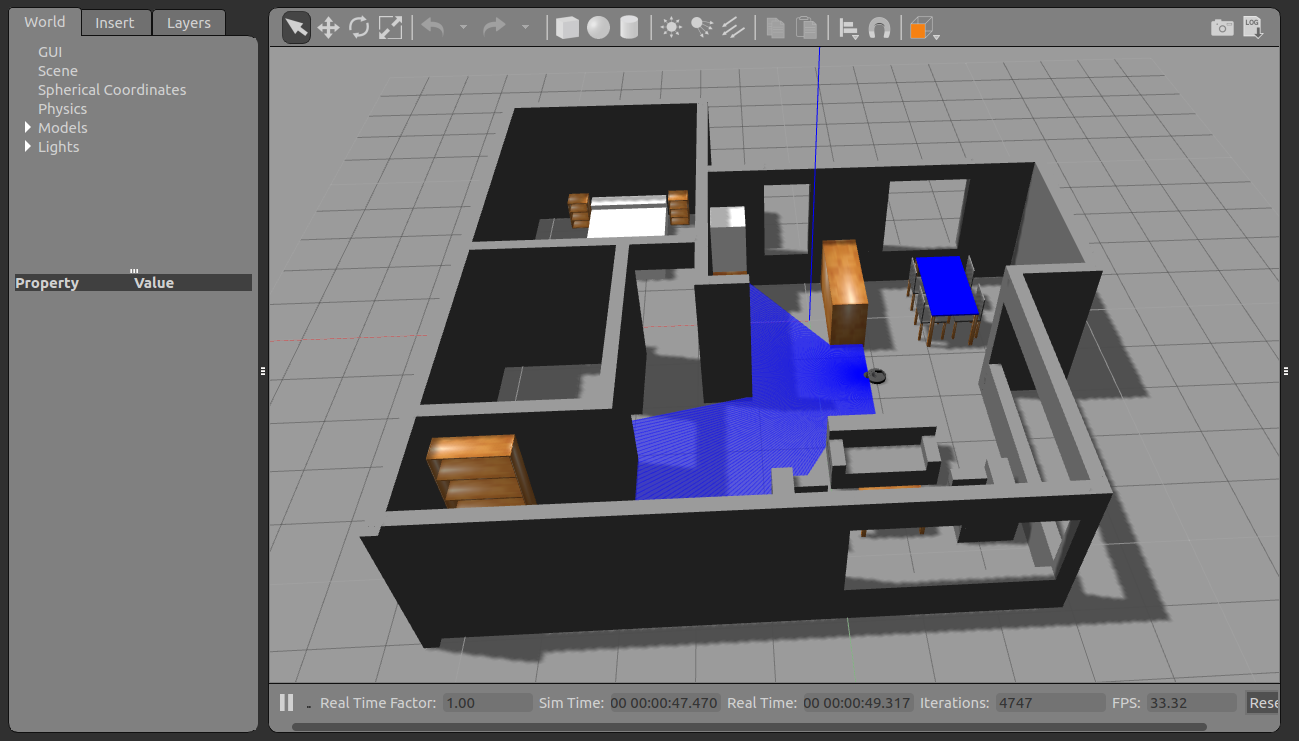
\includegraphics[width=0.9\textwidth]{figures/Infraestructura/gazebo.png}
		\caption{Simulador Gazebo}
		\label{fig.gazebo}
		\end{center}
\end{figure}
 
Gazebo es un programa de código abierto distribuido bajo licencia de Apache 2.0. Se emplea en el desarrollo de aplicaciones robóticas y en inteligencia artificial. Es capaz de simular robots, objetos y sensores en entornos complejos de interior y exterior. Tiene gráficos de gran calidad y un robusto motor de física (masa del robot, rozamiento, inercia, amortiguamiento, etc.). En la Figura~\ref{fig.gazebo} aparece el mundo utilizado en la práctica de ``Aspiradora autónoma con autolocalización''. Se puede apreciar como Gazebo simula tanto objetos (camas, sofás, muebles...) como robots, en este caso, un robot aspirador. \\

Fue elegido para realizar el DARPA Robotics Challenge (2012-2015) y está mantenido por la Fundación Robótica de Código Abierto (OSRF). \\

En este proyecto se emplea la versión 7 de Gazebo, la cual se usará para crear los diferentes entornos y para probar nuestros algoritmos.  Gracias a Gazebo se pueden incluir texturas, luces y sombras en los escenarios, así como simular física como por ejemplo choques, empujes, gravedad, etc. Además, incluye diversos sensores, como pueden ser cámaras y lásers, los cuales podrán ser incorporados en los robots que empleemos. Todo ello hace que sea una herramienta muy potente y de gran ayuda en el mundo de la robótica.\\

Los mundos simulados con Gazebo son 3D, que se cargan a partir de ficheros con extensión ``.world''. Son ficheros definidos en \acrfull{sdf} que es un formato \acrshort{xml} que describe objetos y entornos para simuladores, visualización y control de robots. Originalmente fue desarrollado como parte del simulador Gazebo pero con los años se ha convertido en un formato estable, robusto y extensible capaz de describir todos los aspectos de los robots, los objetos estáticos y dinámicos, la iluminación, el terreno e incluso la física.\\

Se puede describir con precisión todos los aspectos de un robot que usa \acrshort{sdf}, ya sea un robot que sea un simple chasis con ruedas o un humanoide. Además de los atributos cinemáticos y dinámicos, se pueden definir sensores, propiedades de superficie, texturas, fricción de la junta y muchas más propiedades para un robot. Estas características permiten usar \acrshort{sdf} para simulación, visualización, planificación de movimiento y control de robot. Los modelos de robots que se emplean en la simulación pueden ser creados mediante algún programa de modelado 3D como Blender o Sketchup. Estos robots simulados necesitan ser dotados de inteligencia para lo cual se emplean plugins. Éstos, pueden dotar al robot de inteligencia u ofrecer la información de sus sensores a aplicaciones externas y recibir de éstas comandos para los actuadores de los robots.


\section{Entorno JdeRobot}

JdeRobot \footnote{\url{http://jderobot.org/Main_Page}} es un middleware de software libre para el desarrollo de aplicaciones con robots y visión artificial. Esta plataforma fue creada por el Grupo de Robótica de la Universidad Rey Juan Carlos en 2003 y está licenciada como GPLv3 \footnote{\url{https://www.gnu.org/licenses/quick-guide-gplv3.html}}.\\

Está desarrollado en C y C++, aunque contiene componentes desarrollados en lenguajes como Python y Java. Proporciona un entorno de programación distribuido basado en componentes, donde el programa de aplicación se compone de una colección de varios componentes concurrentes asincrónicos. Dichos componentes operan entre sí mediante el middleware de comunicación \acrshort{ice}, que permite la interoperación incluso estando desarrollados en diferentes lenguajes, o \acrshort{ros}messages. Los componentes pueden tener su propia \acrfull{gui}.

La obtención de mediciones del sensor u órdenes del motor se realizan llamando a funciones locales que se encuentran en los drivers. La plataforma conecta esas llamadas a componentes del controlador que están conectados a dispositivos hardware del robot (reales o simulados, remotos o locales). Esas funciones crean la \acrfull{api} para la capa de abstracción de hardware. \\

Las aplicaciones constan de uno o varios componentes. Los que interactúan directamente con los sensores y actuadores del robot se llaman drivers, que son los encargados de controlar que los robots reciben órdenes a través de interfaces \acrshort{ice} o \acrshort{ros} messages. Otros llevan en su código las funciones perceptivas, procesamiento de señales o la lógica de control e inteligencia del robot. En la siguiente imagen se puede ver un ejemplo de esta comunicación con un AR Drone empleando interfaces \acrshort{ice}. La misma lógica de comportamiento se puede conectar al driver del drone real o al drive del drone simulado, basta con cambiar la configuración.

\begin{figure}[H]
  \begin{center}
    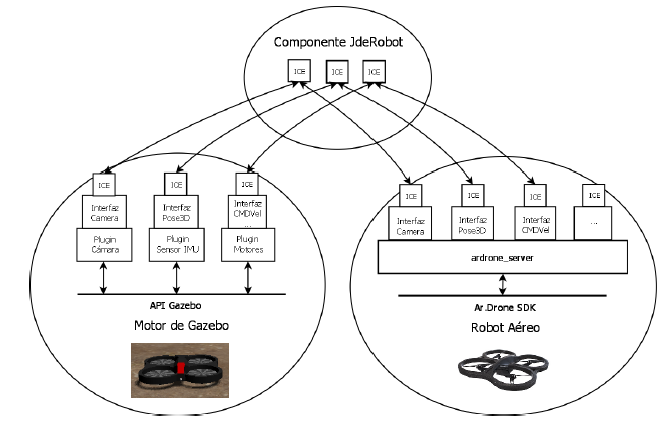
\includegraphics[width=0.9\textwidth]{figures/Infraestructura/jderobot.png}
		\caption{Ejemplo de componentes JdeRobot }
		\label{fig.jderobot}
		\end{center}
\end{figure}

Algunos de los dispositivos y robots actualmente compatibles con JdeRobot son:
\begin{itemize}
	\item Sensores RGBD: Kinect y Kinect2 de Microsoft, Asus Xtion
	\item Robots de ruedas: TurtleBot de Yujin Robot y Pioneer de MobileRobotics Inc.
	\item ArDrone quadrotor de Parrot
	\item Escáneres láser: LMS de SICK, URG de Hokuyo y RPLidar
	\item Cámaras Firewire, cámaras USB, archivos de vídeo (mpeg, avi ...), cámaras IP (como Axis)
\end{itemize}


JdeRobot también incluye varias herramientas y bibliotecas de programación de robots como:
\begin{itemize}
	\item Teleoperadores para varios robots, viendo sus sensores y controlando sus motores. 
	\item Herramienta ``VisualStates'' para programar el comportamiento del robot.
	\item Herramienta ``Scratch2JdeRobot'' para programar robots (incluidos los drones) con el lenguaje gráfico estándar.
	\item Un calibrador de cámara.
	\item Una herramienta para filtros de color.
	\item Una biblioteca para desarrollar controladores y una biblioteca para la geometría proyectiva y el procesamiento de visión artificial.
\end{itemize}

En el desarrollo del proyecto se empleará la versión 5.6.2 de JdeRobot, ya que es la última versión estable.

\section{Lenguaje de programación Python}

Paython \footnote{\url{https://www.python.org/}}, como se argumentó en el Capítulo 1, es uno de los ejes principales de JdeRobot-Academy. Es el lenguaje de programación en el que están escritos los componentes académicos y las soluciones por lo que es el lenguaje utilizado para el desarrollo de este proyecto. Se trata de un lenguaje fácil de aprender y de alto nivel, es decir, se caracteriza por expresar los algoritmos de una manera adecuada a la capacidad cognitiva humana. Su creador fue Guido van Rossum, un investigador holandés que trabajaba en el centro de investigación CWI (Centrum Wiskunde \& Informatica).\\

Algunas funcionalidades incluidas en Python son la programación orientada a objetos, el manejo de excepciones, listas y diccionarios entre otras. A pesar de todo lo que soporta, se creó con el objetivo de que fuera un lenguaje sencillo de entender, sin perder todas las funcionalidades que pueden ofrecer lenguajes complejos tales como C.\\

Actualmente Python se trata de un lenguaje de código abierto administrado por Python Software Foundation. Este lenguaje incluye módulos que permiten la entrada y salida de ficheros, sockets, llamadas al sistema e incluso interfaces gráficas como Qt. Además, permite dividir el programa en módulos reutilizables y no es necesario compilarlo, pues es un lenguaje de programación interpretado. \\

La última versión ofrecida por Python Software Foundation es la 3.6.2, pero en nuestro caso se empleará la 2.7.12 por compatibilidad con JdeRobot 5.5.2, que a su vez, sigue en esa versión de Python para ser compatible con \acrshort{ros} Kinetic.


\section{Biblioteca OpenCV}
OpenCV \footnote{\url{http://opencv.org/}} es una librería de código abierto desarrollada por Intel y publicada bajo licencia de BSD. Sus siglas provienen de los términos anglosajones ``Open Source Computer Vision Library''. Esta librería implementa gran variedad de herramientas para la interpretación de la imagen.\\

Los algoritmos se basan en estructuras de datos flexibles acopladas con estructuras IPL (Intel Image Processing Library), aprovechándose de la arquitectura de Intel en la optimización de más de la mitad de las funciones. \\

La biblioteca cuenta con más de 2500 algoritmos optimizados, que incluyen un conjunto completo de algoritmos de visión artificial y de aprendizaje automático, tanto clásicos como avanzados. Estos algoritmos se pueden usar para detectar y reconocer rostros, identificar objetos, rastrear movimientos de la cámara, rastrear objetos en movimiento, extraer modelos 3D de objetos, unir imágenes para producir una alta resolución imagen de una escena completa, encontrar imágenes similares de una base de datos de imágenes, etc. También tiene una librería de aprendizaje automático (MLL, Machine Learning Library) destinada al reconocimiento y agrupación de patrones estadísticos. \\

Fue diseñado para tener una alta eficiencia computacional. Está escrito en C/C++ y puede aprovechar las ventajas de los procesadores multinúcleo. Los algoritmos se basan en estructuras de datos flexibles acopladas con estructuras IPL (Intel Image Processing Library), aprovechándose de la arquitectura de Intel en la optimización de más de la mitad de las funciones. \\

Desde su aparición OpenCV ha sido usado en numerosas aplicaciones entre las cuales se encuentran la unión de imágenes de satélites y de mapas web, la reducción de ruido en imágenes médicas, los sistemas de detección de movimiento, la calibración de cámaras, el manejo de vehículos no tripulados o el reconocimiento de gestos. OpenCV es empleado también en reconocimiento de música y sonido, mediante la aplicación de técnicas de reconocimiento de visión en imágenes de espectrogramas del sonido.\\

OpenCV ha sido usada en el sistema de visión del vehículo no tripulado Stanley de la Universidad de Stanford, el ganador en el año 2005 del Gran desafío DARPA. \\

Hay una gran cantidad de empresas y centros de investigación que emplean estas técnicas como IBM, Microsoft, Intel, SONY, Siemens, Google, Stanford, MIT, CMU, Cambridge e INRIA.\\

Esta librería puede ser usada en distintos sistemas operativos como MAC, Windows, Android y Linux, y existen versiones para lenguajes de programación como C\#, Python y Java, a pesar de que originalmente era una librería en C/C++. Además, hay interfaces en desarrollo para Ruby, Matlab y otros lenguajes.\\

En este trabajo se ha empleado la versión 3.2 de OpenCV en Python. Esta librería se empleará para realizar todo lo relacionado con el tratamiento digital de imágenes. Con ello se extraerán datos que puedan emplearse a la hora de tomar decisiones para que los robots funcionen correctamente.

\section{PyQt}
PyQt es un conjunto de enlaces Python para el conjunto de herramientas Qt, las cuales se emplean para el desarrollo de interfaces gráficas. Fue desarrollado por Riverbank Computing Ltd y es soportado por Windows, Linux, Mac OS/X, iOS y Android.\\

Qt es un entorno multiplataforma orientado a objetos desarrollado en C++  que permite desarrollar interfaces gráficas e incluye sockets, hilos, Unicode, bases de datos SQL, etc. PyQt combina todas las ventajas de Qt y Python, pues permite emplear todas las funcionalidades ofrecidas por Qt con un lenguaje de programación tan sencillo como Python.\\

PyQt5 es un conjunto de enlaces Python para Qt5, disponible en Python 2.x y 3.x. Tiene más de 620 clases y 6000 funciones y métodos. PyQt5 dispone de una licencia dual, es decir, los desarrolladores pueden elegir entre una licencia GPL (General Public Licence) o una licencia comercial.\\ 

La interfaz gráfica de los componentes académicos creados en las prácticas está escrita usando PyQt5. Las clases se dividen en ciertos módulos, tales como QtCore, QtGui, QtWidgets, QtXml o QtSql. En las prácticas desarrolladas se ha hecho uso de los siguientes módulos:
\begin{itemize}
	\item QtCore: contiene las funcionalidades principales que no tienen que ver con la interfaz gráfica. Este módulo se emplea para trabajar con archivos, diferentes tipos de datos, hilos, procesos, url, etc.
	\item QtGui: contiene clases para el desarrollo de ventanas, gráficos 2D, imágenes y texto.
	\item QtWidgets: dispone de clases que proporcionan un conjunto de elementos de interfaz de usuario para crear interfaces de usuario clásicas de escritorio. 
\end{itemize}

En este proyecto se ha empleado PyQt5, la versión 5 de PyQt. 
